\appendix
\section{Appendices}

\subsection{Additional Explanations}

\subsection{Defining Matthew's Correlation Coefficient}\label{appendix:matthews_correlation}
$$\mathrm{MCC} = \frac{\mathrm{TP}\cdot\mathrm{TN}-\mathrm{FP}\cdot\mathrm{FN}}{\sqrt{(\mathrm{TP}+\mathrm{FP})\cdot(\mathrm{TP}+\mathrm{FN})\cdot(\mathrm{TN}+\mathrm{FP})\cdot(\mathrm{TN})+\mathrm{FN}}}$$ 
The values of MCC are bounded within the range $[-1;1]$, where 1 represents a perfect prediction, 0 represents random prediction and -1 total disagreement between prediction and observation. Refer to \cite{chicco_jurman_2020_mcc_f1} regarding the necessary normalization to make the MCC values bounded within $[0;1]$ so that they can be plotted against F1 scores (which themselves are bounded in $[0;1]$)

\subsubsection{Deriving the Frames Per Person in the Caltech Dataset}\label{appendix:caltech_frames_per_person}
The total running time of the Caltech videos is $\sim 10\mathrm{h}$ \cite{dollar_2009_pedestrian}, this gives a frame per second rate of $\sim 7 \text{ frames}/\mathrm{s}$. Since a person is present in a video for $\sim 5 \mathrm{s}$ \cite{dollar_2009_pedestrian}, we can approximate that each identifiable individual will, on average, be present in $34 \text{ frames}$
\subsubsection{Choice of Grayscale Conversion}\label{appendix:grayscale_discuss}
The primary motivation behind the simple color mapping in equation \ref{eq:colour_map} is the wide adoption in image processing libraries, such as \href{https://scikit-image.org/}{scikit-image}. While there are more sophisticated methods of RGB to grayscale conversion \cite{madk_2008_perceptual}, the computational overhead is difficult to justify given the the rather ambiguous nature of assessing which specific color space transformation produces universally desirable outputs for all involved input images \cite{madk_2008_perceptual}.
\subsection{Python Code Implementations}
\subsubsection{Grayscale Transformation}\label{appendix:grayscale}
\begin{pythoncode}
from skimage.color import rgb2gray
import numpy as np
from tqdm import tqdm
def grayscale_transform(X):
    '''
    Convert a collection of RGB images to grayscale.

    Parameters:
    -----------
    X : list or np.ndarray
        A collection of RGB images, where each image is represented as a 3D array (height x width x channels).

    Returns:
    --------
    np.ndarray
        A 3D numpy array containing the grayscale versions of the input images, 
        where each grayscale image is represented as a 2D array (height x width).
    '''
    return np.array([rgb2gray(img) for img in tqdm(X)])
\end{pythoncode}
\subsubsection{Central Differences Derivative Mask}
\begin{pythoncode}
from skimage.feature._hog _hog_channel_gradient
def _central_hog_channel_gradient(channel):
    return _hog_channel_gradient(channel)
\end{pythoncode}

\subsubsection{Holistic Derivative Mask}\label{appendix:holistic_der_mask}
\begin{pythoncode}
import numpy as np

def _holistic_hog_channel_gradient(channel):
    '''
    Compute the gradients of a single channel using forward, backward, and central difference methods.

    Parameters:
    -----------
    channel : np.ndarray
        A 2D numpy array representing a single channel of an image.

    Returns:
    --------
    g_row : np.ndarray
        A 2D numpy array containing the gradient along the rows.
    
    g_col : np.ndarray
        A 2D numpy array containing the gradient along the columns.
    '''
    g_row = np.zeros(channel.shape, dtype=channel.dtype)
    g_col = np.zeros(channel.shape, dtype=channel.dtype)
    # forward difference
    g_row[0, :] = channel[1, :] - channel[0, :]
    g_col[:, 0] = channel[:, 1] - channel[:, 0]
    # backward difference
    g_row[-1, :] = channel[-1, :] - channel[-2, :]
    g_col[:, -1] = channel[:, -1] - channel[:, -2]
    # central difference
    g_row[1:-1, :] = (channel[2:, :] - channel[:-2, :])
    g_col[:, 1:-1] = (channel[:, 2:] - channel[:, :-2])

    return g_row, g_col
\end{pythoncode}
\subsubsection{Modified HOG Computation}\label{appendix:hog}
\begin{pythoncode}
def hog(
        image,
        hog_parameters: HOG_Parameters
):
    '''
    Compute the Histogram of Oriented Gradients (HOG) for the input image.

    Parameters:
    -----------
    image : np.ndarray
        A 2D numpy array representing the input image.
    
    hog_parameters : HOG_Parameters
        An object containing parameters for the HOG computation, including:
        - pixels_per_cell: Tuple specifying the size of the cells.
        - cells_per_block: Tuple specifying the number of cells per block.
        - block_stride: Tuple specifying the stride between blocks.
        - orientations: Number of orientation bins.
        - holistic_derivative_mask: Boolean to determine the gradient calculation method.
    
    Returns:
    --------
    np.ndarray
        A 1D numpy array containing the normalized HOG features for the input image.
    
    Raises:
    -------
    ValueError
        If the input image does not have two spatial dimensions or is too small
        given the specified parameters.
    '''

    image = np.atleast_2d(image)
    float_dtype = utils._supported_float_type(image.dtype)
    image = image.astype(float_dtype, copy=False)

    if image.ndim != 2:
        raise ValueError(
            'Only images with two spatial dimensions are supported.'
        )

    g_row, g_col = _holistic_hog_channel_gradient(
        image) if hog_parameters.holistic_derivative_mask else _central_hog_channel_gradient(
        image)

    s_row, s_col = image.shape[:2]
    c_row, c_col = hog_parameters.pixels_per_cell
    b_row, b_col = hog_parameters.cells_per_block
    b_row_stride, b_col_stride = hog_parameters.block_stride

    n_cells_row = int(s_row // c_row)
    n_cells_col = int(s_col // c_col)

    orientation_histogram = np.zeros(
        (n_cells_row, n_cells_col, hog_parameters.orientations), dtype=float
    )
    g_row = g_row.astype(float, copy=False)
    g_col = g_col.astype(float, copy=False)

    _hoghistogram.hog_histograms(
        g_col,
        g_row,
        c_col,
        c_row,
        s_col,
        s_row,
        n_cells_col,
        n_cells_row,
        hog_parameters.orientations,
        orientation_histogram,
    )

    n_blocks_row = (s_row - (b_row + 1) * c_row) // (b_row_stride * c_row)
    n_blocks_col = (s_col - (b_col + 1) * c_col) // (b_col_stride * c_col)
    if n_blocks_col <= 0 or n_blocks_row <= 0:
        min_row = b_row * c_row
        min_col = b_col * c_col
        raise ValueError(
            'The input image is too small given the values of '
            'pixels_per_cell and cells_per_block. '
            'It should have at least: '
            f'{min_row} rows and {min_col} cols.'
        )
    normalized_blocks = np.zeros(
        (n_blocks_row, n_blocks_col, b_row, b_col, hog_parameters.orientations), dtype=float_dtype
    )

    for r in range(0, n_blocks_row):
        for c in range(0, n_blocks_col):
            block = orientation_histogram[
                    r * b_row_stride: r * b_row_stride + b_row,  
                    c * b_col_stride: c * b_col_stride + b_col,  
                    :
                    ]
            normalized_blocks[r, c, :] = _hog_normalize_block(block, method=hog_parameters.block_norm)
    normalized_blocks = normalized_blocks.ravel()

    return normalized_blocks
    
def hog_transform(X, hog_parameters: HOG_Parameters):
    '''
    Apply the Histogram of Oriented Gradients (HOG) transformation to a collection of images.

    Parameters:
    -----------
    X : list or np.ndarray
        A collection of images, where each image is represented as a 2D numpy array.
    
    hog_parameters : HOG_Parameters
        An object containing parameters for the HOG computation.
    
    Returns:
    --------
    np.ndarray
        A 2D numpy array containing the HOG features for each input image, 
        with each row representing the features of an individual image.
    '''
    return np.array([hog(img,hog_parameters) for img in tqdm(X)])
    
\end{pythoncode}
\subsubsection{Caltech Data Set Transformation}\label{appendix:caltech_transform}
\begin{pythoncode}
import os, glob
import cv2
from scipy.io import loadmat
from collections import defaultdict
import numpy as np
from lxml import etree, objectify

def vbb_anno2dict(vbb_file, cam_id, person_types=None):
    """
    Parse caltech vbb annotation file to dict
    Args:
        vbb_file: input vbb file path
        cam_id: camera id
        person_types: list of person type that will be used (total 4 types: person, person-fa, person?, people).
            If None, all will be used:
    Return:
        Annotation info dict with filename as key and anno info as value
    """
    filename = os.path.splitext(os.path.basename(vbb_file))[0]
    annos = defaultdict(dict)
    vbb = loadmat(vbb_file)
    # object info in each frame: id, pos, occlusion, lock, posv
    objLists = vbb['A'][0][0][1][0]
    objLbl = [str(v[0]) for v in vbb['A'][0][0][4][0]]
    # person index
    if not person_types:
        person_types = ["person", "person-fa", "person?", "people"]
    person_index_list = [x for x in range(len(objLbl)) if objLbl[x] in person_types]
    for frame_id, obj in enumerate(objLists):
        if len(obj) > 0:
            frame_name = str(cam_id) + "_" + str(filename) + "_" + str(frame_id+1) + ".jpg"
            annos[frame_name] = defaultdict(list)
            annos[frame_name]["id"] = frame_name
            for fid, pos, occl in zip(obj['id'][0], obj['pos'][0], obj['occl'][0]):
                fid = int(fid[0][0]) - 1  # for matlab start from 1 not 0
                if not fid in person_index_list:  # only use bbox whose label is given person type
                    continue
                annos[frame_name]["label"] = objLbl[fid]
                pos = pos[0].tolist()
                occl = int(occl[0][0])
                annos[frame_name]["occlusion"].append(occl)
                annos[frame_name]["bbox"].append(pos)
            if not annos[frame_name]["bbox"]:
                del annos[frame_name]
    return annos


def seq2img(annos, seq_file, outdir, cam_id):
    """
    Extract frames in seq files to given output directories
    Args:
         annos: annos dict returned from parsed vbb file
         seq_file: seq file path
         outdir: frame save dir
         cam_id: camera id
    Returns:
        camera captured image size
    """
    cap = cv2.VideoCapture(seq_file)
    index = 1
    # captured frame list
    v_id = os.path.splitext(os.path.basename(seq_file))[0]
    cap_frames_index = np.sort([int(os.path.splitext(id)[0].split("_")[2]) for id in annos.keys()])
    while True:
        ret, frame = cap.read()
        if ret:
            if not index in cap_frames_index:
                index += 1
                continue
            if not os.path.exists(outdir):
                os.makedirs(outdir)
            outname = os.path.join(outdir, str(cam_id)+"_"+v_id+"_"+str(index)+".jpg")
            print("Current frame: ", v_id, str(index))
            cv2.imwrite(outname, frame)
            height, width, _ = frame.shape
        else:
            break
        index += 1
    img_size = (width, height)
    return img_size


def instance2xml_base(anno, img_size, bbox_type='xyxy'):
    """
    Parse annotation data to VOC XML format
    Args:
        anno: annotation info returned by vbb_anno2dict function
        img_size: camera captured image size
        bbox_type: bbox coordinate record format: xyxy (xmin, ymin, xmax, ymax); xywh (xmin, ymin, width, height)
    Returns:
        Annotation xml info tree
    """
    assert bbox_type in ['xyxy', 'xywh']
    E = objectify.ElementMaker(annotate=False)
    anno_tree = E.annotation(
        E.folder('VOC2014_instance/person'),
        E.filename(anno['id']),
        E.source(
            E.database('Caltech pedestrian'),
            E.annotation('Caltech pedestrian'),
            E.image('Caltech pedestrian'),
            E.url('None')
        ),
        E.size(
            E.width(img_size[0]),
            E.height(img_size[1]),
            E.depth(3)
        ),
        E.segmented(0),
    )
    for index, bbox in enumerate(anno['bbox']):
        bbox = [float(x) for x in bbox]
        if bbox_type == 'xyxy':
            xmin, ymin, w, h = bbox
            xmax = xmin+w
            ymax = ymin+h
        else:
            xmin, ymin, xmax, ymax = bbox
        xmin = int(xmin)
        ymin = int(ymin)
        xmax = int(xmax)
        ymax = int(ymax)
        if xmin < 0:
            xmin = 0
        if xmax > img_size[0] - 1:
            xmax = img_size[0] - 1
        if ymin < 0:
            ymin = 0
        if ymax > img_size[1] - 1:
            ymax = img_size[1] - 1
        if ymax <= ymin or xmax <= xmin:
            continue
        E = objectify.ElementMaker(annotate=False)
        anno_tree.append(
            E.object(
            E.name(anno['label']),
            E.bndbox(
                E.xmin(xmin),
                E.ymin(ymin),
                E.xmax(xmax),
                E.ymax(ymax)
            ),
            E.difficult(0),
            E.occlusion(anno["occlusion"][index])
            )
        )
    return anno_tree


def parse_anno_file(vbb_inputdir, seq_inputdir, vbb_outputdir, seq_outputdir, person_types=None):
    """
    Parse Caltech data stored in seq and vbb files to VOC xml format
    Args:
        vbb_inputdir: vbb file saved pth
        seq_inputdir: seq file saved path
        vbb_outputdir: vbb data converted xml file saved path
        seq_outputdir: seq data converted frame image file saved path
        person_types: list of person type that will be used (total 4 types: person, person-fa, person?, people).
            If None, all will be used:
    """
    # annotation sub-directories in hda annotation input directory
    assert os.path.exists(vbb_inputdir)
    sub_dirs = os.listdir(vbb_inputdir)
    for sub_dir in sub_dirs:
        print("Parsing annotations of camera: ", sub_dir)
        cam_id = sub_dir
        vbb_files = glob.glob(os.path.join(vbb_inputdir, sub_dir, "*.vbb"))
        for vbb_file in vbb_files:
            annos = vbb_anno2dict(vbb_file, cam_id, person_types=person_types)
            if annos:
                vbb_outdir = os.path.join(vbb_outputdir, "annotations", sub_dir, "bbox")
                # extract frames from seq
                seq_file = os.path.join(seq_inputdir, sub_dir, os.path.splitext(os.path.basename(vbb_file))[0]+".seq")
                seq_outdir = os.path.join(seq_outputdir, sub_dir, "frame")
                if not os.path.exists(vbb_outdir):
                    os.makedirs(vbb_outdir)
                if not os.path.exists(seq_outdir):
                    os.makedirs(seq_outdir)
                img_size = seq2img(annos, seq_file, seq_outdir, cam_id)
                for filename, anno in sorted(annos.items(), key=lambda x: x[0]):
                    if "bbox" in anno:
                        anno_tree = instance2xml_base(anno, img_size)
                        outfile = os.path.join(vbb_outdir, os.path.splitext(filename)[0]+".xml")
                        print("Generating annotation xml file of picture: ", filename)
                        etree.ElementTree(anno_tree).write(outfile, pretty_print=True)

def main():    
    seq_dir = "Pedestrian-Detection/datasets/caltech_raw/Test"
    vbb_dir = "Pedestrian-Detection/datasets/caltech_raw/annotations/Test"
    out_dir = "Pedestrian-Detection/datasets/caltech_parsed/Test"
    frame_out = os.path.join(out_dir, "frame")
    anno_out = os.path.join(out_dir, "annotation")
    person_type = ["person", "people"]
    parse_anno_file(vbb_dir, seq_dir, frame_out, anno_out, person_type)
\end{pythoncode}
\subsubsection{Retain 30th Caltech Data Set Frame}\label{appendix:caltech_30_frame}
\begin{pythoncode}
import os
from tqdm import tqdm
def retain_30th_frame():
    root_dir = r'/Users/adamsam/repos/ee/Pedestrian-Detection/datasets/caltech_30/Test'
    annotation_dir = os.path.join(root_dir, 'annotations')
    frame_dir = os.path.join(root_dir, 'frame')
    frame_instance = 0
    for frame_subdir in tqdm(os.listdir(frame_dir)):
        frame_subdir_path = os.path.join(frame_dir, frame_subdir)
        if(os.path.isdir(frame_subdir_path)):
            frame_files = os.listdir(os.path.join(frame_subdir_path, 'frame'))
            for frame_file in frame_files:
                file_location = os.path.join(frame_subdir_path, 'frame', frame_file)
    
                if not os.path.isfile(file_location):
                    continue
    
                if frame_instance % 30 != 0:
                    os.remove(file_location)
                    annotation_file_location = os.path.join(annotation_dir, frame_subdir, 'bbox', frame_file.split('.')[0] + '.xml')
                    if os.path.isfile(annotation_file_location):
                        os.remove(annotation_file_location)
                frame_instance += 1
\end{pythoncode}
\subsubsection{Pedestrian Data Set Construction}\label{appendix:dataset}
\begin{pythoncode}
import cv2
import numpy as np
import os
from sklearn.model_selection import train_test_split
from tqdm import tqdm
import random

window_sizes = [(128, 64), (112, 48), (100, 50), (128, 96)]

class SampleCount:
    def __init__(self, pos_count, neg_count):
        '''
        Initialize the SampleCount object.

        Parameters:
        -----------
        pos_count : int
            The number of positive samples.
        
        neg_count : int
            The number of negative samples.
        '''
        self.pos = pos_count
        self.neg = neg_count

class LabeledDataSet:
    def __init__(self, points, labels, sample_count: SampleCount):
        '''
        Initialize the LabeledDataSet object.

        Parameters:
        -----------
        points : np.ndarray
            The data points (images) in the dataset.
        
        labels : np.ndarray
            The corresponding labels for the data points.
        
        sample_count : SampleCount
            An object containing the counts of positive and negative samples.
        '''
        self.points = points
        self.labels = labels
        self.sample_count = sample_count

def parse_pascal_voc_annotations(file_name):
    '''
    Parse Pascal VOC annotations from an XML file.

    Parameters:
    -----------
    file_name : str
        The path to the annotation XML file.

    Returns:
    --------
    list
        A list of bounding boxes, each represented as a list of integers [xmin, ymin, xmax, ymax].
    '''
    import xml.etree.ElementTree as ET
    tree = ET.parse(file_name)
    root = tree.getroot()
    bbox = []

    for obj in root.findall('object'):
        bndbox = obj.find('bndbox')
        bbox.append([
            int(bndbox.find('xmin').text),
            int(bndbox.find('ymin').text),
            int(bndbox.find('xmax').text),
            int(bndbox.find('ymax').text)
        ])
    return bbox


def prepare_labeled_datasets(image_folder, window_size, test_size=0.2, random_state=42):
    '''
    Prepare labeled datasets for training and testing.

    Parameters:
    -----------
    image_folder : str
        The path to the folder containing images and annotations.
    
    window_size : tuple
        The size of the sliding window for sample extraction.
    
    test_size : float
        The proportion of the dataset to include in the test split (default is 0.2).
    
    random_state : int
        Random seed for reproducibility (default is 42).

    Returns:
    --------
    LabeledDataSet, LabeledDataSet
        The training and testing labeled datasets.
    '''
    image_dir = os.path.join(image_folder, "frame")
    annotation_dir = os.path.join(image_folder, "annotations")

    image_subdirs = [
        os.path.join(image_dir, subdir)
        for subdir in os.listdir(image_dir)
        if os.path.isdir(os.path.join(image_dir, subdir))
    ]
    images = [os.path.join(subdir, file) for subdir in image_subdirs for file in os.listdir(subdir) if
              os.path.isfile(os.path.join(subdir, file))]


    train_images, test_images = train_test_split(images, test_size=test_size, random_state=random_state)

    def process_images(image_list):
        data_points = []
        labels = []
        num_pos = 0
        num_neg = 0

        for num, image_file_location in enumerate(tqdm(image_list)):
            image = cv2.imread(image_file_location)

            partial_location = image_file_location.split(os.sep)[-2:]
            annotation_file_location = os.path.join(
                annotation_dir,
                "/".join(map(str, partial_location))
            )[:-4]

            if os.path.exists(annotation_file_location + ".xml"):
                bbox_arr = parse_pascal_voc_annotations(annotation_file_location + ".xml")
            else:
                raise Exception(f"Annotation file {annotation_file_location} not found")

            for _ in range(3):
                h, w = image.shape[:2]

                if h > window_size[0] or w > window_size[1]:
                    h = h - window_size[0]
                    w = w - window_size[1]
                    max_loop = 0
                    overlap = []
                    new_window = []
                    for _ in range(10):
                        x = random.randint(0, w)
                        y = random.randint(0, h)
                        overlap = [True for i in bbox_arr]
                        new_window = [x, y, x + window_size[1], y + window_size[0]]
                        
                        for index, bbox in enumerate(bbox_arr):
                            dx = min(bbox[2], new_window[2]) - max(bbox[0], new_window[0])
                            dy = min(bbox[3], new_window[3]) - max(bbox[1], new_window[1])
                            if dx <= 0 or dy <= 0:
                                overlap[index] = False
                        if not np.any(overlap):
                            break
                    if not np.any(overlap):
                        img = image[window[1]:window[3], window[0]:window[2]]
                        data_points.append(img)
                        labels.append(0)
                        num_neg += 1

            # Process positive samples (bounding boxes)
            for box in bbox_arr:
                upper_random_boundary = random.randint(5,20)
                pad_left = random.randint(0, upper_random_boundary)
                pad_right = random.randint(0, upper_random_boundary)
                pad_top = random.randint(0, upper_random_boundary)
                pad_bottom = random.randint(0, upper_random_boundary)
                x1 = box[0] + pad_left
                y1 = box[1] + pad_top
                x2 = box[2] - pad_right
                y2 = box[3] - pad_bottom
                if x1 > x2:
                    x2 = min(image.shape[1], box[2] + pad_left)
                if y1 > y2:
                    y2 = min(image.shape[0],box[3]+pad_top)
                img = image[y1:y2, x1:x2]
                img_resized = cv2.resize(img, (window_size[1], window_size[0]))
                data_points.append(img_resized)
                labels.append(1)
                num_pos += 1


        return data_points, labels, num_pos, num_neg

    train_data, train_labels, train_pos, train_neg = process_images(train_images)
    test_data, test_labels, test_pos, test_neg = process_images(test_images)


    labeled_training_set = LabeledDataSet(np.array(train_data), np.array(train_labels), SampleCount(train_pos, train_neg))
    labeled_testing_set = LabeledDataSet(np.array(test_data), np.array(test_labels), SampleCount(test_pos, test_neg))

    return labeled_training_set, labeled_testing_set


def get_dataset_path(window_size, category, data_type, dataset=None):
    '''
    Get the file path for the dataset based on the window size, category, and data type.

    Parameters:
    -----------
    window_size : tuple
        The size of the sliding window as (height, width).
    
    category : str
        The category of the dataset, either 'train' or 'test'.
    
    data_type : str
        The type of data, either 'point' or 'label'.
    
    dataset : str, optional
        The name of the dataset (required if category is 'test').

    Returns:
    --------
    str
        The file path for the specified dataset.
    '''

    file_path = ''

    if category not in ['train', 'test']:
        raise ValueError('category must be either "train" or "test"')
    if data_type not in ['point', 'label']:
        raise ValueError('data_type must be either "point" or "label"')

    category_dir = f'datasets/npy_{category}'

    file_name = f'{data_type}_{window_size[1]}-{window_size[0]}.npy'

    if category == 'train':
        file_path = os.path.join(category_dir, file_name)
    elif category == 'test' and dataset is not None:
        file_path = os.path.join(category_dir, dataset, file_name)

    if not os.path.exists(os.path.dirname(file_path)):
        os.makedirs(os.path.dirname(file_path))

    return file_path


def init_datasets(datasets_path):
    '''
    Initialize datasets for different window sizes and save the training and testing sets.

    Parameters:
    -----------
    datasets_path : str
        The path to the datasets directory.
    '''
    for window_size in window_sizes:
        total_training_points = np.array([])
        total_training_labels = np.array([])
        for dataset in ['INRIA', 'caltech_30', 'PnPLO']:
            print(f'\n\nInitializing dataset {dataset} with window size {window_size}\n')
            training_set, testing_set = prepare_labeled_datasets(os.path.join(datasets_path, dataset), window_size)

            print("Training Positives: ", training_set.sample_count.pos)
            print("Training Negatives: ", training_set.sample_count.neg)
            print("Testing Positives: ", testing_set.sample_count.pos)
            print("Testing Negatives: ", testing_set.sample_count.neg)

            # np.concatenate requires identical array dimensions
            if total_training_points.shape[0] == 0:
                total_training_points = training_set.points
                total_training_labels = training_set.labels
            else:
                total_training_points = np.concatenate((total_training_points, training_set.points))
                total_training_labels = np.concatenate((total_training_labels, training_set.labels))

            np.save(get_dataset_path(window_size, 'test', 'point', dataset), testing_set.points)
            np.save(get_dataset_path(window_size, 'test', 'label', dataset), testing_set.labels)

            print("\nInitialized")

        print("\n\nSaving total training sets\n")
        np.save(get_dataset_path(window_size, 'train', 'point'), total_training_points)
        np.save(get_dataset_path(window_size, 'train', 'label'), total_training_labels)

\end{pythoncode}
\subsubsection{Training a Soft Constraint SVM}\label{appendix:training_svm}
\begin{pythoncode}
import os
import joblib
import numpy as np
from hog import HOG_Parameters, hog
from transform import grayscale_transform, hog_transform
from sklearn.svm import SVC

class SVM_Parameters:
    '''
    Class to hold SVM parameters, including HOG parameters and window size.

    Attributes:
    -----------
    hog_parameters : HOG_Parameters
        Parameters for HOG feature extraction.
    
    window_size : tuple
        The size of the sliding window as (height, width).
    '''
    def __init__(self, hog_parameters: HOG_Parameters, window_size):
        self.hog_parameters = hog_parameters
        self.window_size = window_size
    def get_svm_name(self):
        '''
        Get the name of the SVM model based on HOG parameters and window size.

        Returns:
        --------
        str
            The name of the SVM model.
        '''
        return "svm_" + self.hog_parameters.get_hog_name() + "_window_" + str(self.window_size)

def load_svm(svm_parameters: SVM_Parameters, model_dir, custom_name=None):
    '''
    Load an SVM model from the specified directory.

    Parameters:
    -----------
    svm_parameters : SVM_Parameters
        Parameters associated with the SVM model.
    
    model_dir : str
        The directory where the model is stored.
    
    custom_name : str, optional
        A custom name for the model file.

    Returns:
    --------
    object
        The loaded SVM model.
    
    Raises:
    -------
    Exception
        If the model file is not found.
    '''
    model_name = custom_name if custom_name is not None else svm_parameters.get_svm_name()
    model_file_name = os.path.join(model_dir, model_name + ".pkl")
    print(model_file_name)
    if os.path.exists(model_file_name):
        return joblib.load(model_file_name)
    raise Exception("Model not found")

def train_svm(svm_parameters: SVM_Parameters, data_points_location, labels_location, overwrite=False, custom_name=None):
    '''
    Train an SVM model with the given parameters and save it to a file.

    Parameters:
    -----------
    svm_parameters : SVM_Parameters
        Parameters associated with the SVM model.
    
    data_points_location : str
        Path to the file containing training data points.
    
    labels_location : str
        Path to the file containing training labels.
    
    overwrite : bool, optional
        If True, overwrite the existing model.
    
    custom_name : str, optional
        A custom name for the saved model file.
    
    kernel_type : str, optional
        The type of kernel to use for the SVM.
    '''
    from sklearn.linear_model import SGDClassifier
    from sklearn.model_selection import GridSearchCV
    model_name = custom_name if custom_name is not None else svm_parameters.get_svm_name()

    model_file_path = os.path.join(COMPUTED_PATH, 'models', model_name + ".pkl")

    if os.path.exists(model_file_path):
      if overwrite:
        print("Removing existing model")
        os.remove(model_file_path)
      else:
        print("Model already exists")
        model = load_svm(svm_parameters, custom_name=custom_name)
        single_x = np.load(data_points_location)[0]
        single_x_gray = grayscale_transform(np.array([single_x]))
        single_x_hog = hog_transform(single_x_gray, svm_parameters.hog_parameters)
        try:
            model.predict(single_x_hog)
            print("Model loaded successfully")
            return
        except:
            print("Model failed to load, retraining")

    if os.path.exists(data_points_location) and os.path.exists(labels_location):
        training_data_points = np.load(data_points_location)
        training_labels = np.load(labels_location)
    else:
        raise Exception(
            "No data points or labels found",
            data_points_location,
            labels_location
        )

    x_train = np.load(data_points_location)
    y_train = np.load(labels_location)

    x_train_gray = grayscale_transform(x_train)
    x_train_hog = hog_transform(x_train_gray, svm_parameters.hog_parameters)
    
    # Define hyperparameters for optimization
    param_grid = {
        'alpha': [0.0001, 0.001, 0.01, 0.1]
    }

    sgd_clf = SGDClassifier(random_state=42, max_iter=1000, tol=1e-3)
    grid_search = GridSearchCV(sgd_clf, param_grid, cv=5, scoring='matthews_corrcoef', learning_rate="optima" n_jobs=-1)

    grid_search.fit(x_train_hog, y_train)
    best_model = grid_search.best_estimator_

    joblib.dump(best_model, model_file_path)

\end{pythoncode}

\subsubsection{Plotting MCC-F1 Curves}\label{appendix:mcc_f1_curves}
\begin{pythoncode}
from mcc_f1 import mcc_f1_curve
from mcc_f1._plot.base import _get_response

class MCCF1CurveDisplay:
    """MCC-F1 Curve visualization with threshold values."""

    def __init__(self, *, f1, mcc, thresholds,
                 mcc_f1=None, estimator_name=None, pos_label=None):
        self.estimator_name = estimator_name
        self.f1 = f1
        self.mcc = mcc
        self.thresholds = thresholds
        self.mcc_f1 = mcc_f1
        self.pos_label = pos_label

    def plot(self, ax=None, *, name=None, n_thresholds=0, **kwargs):
        """Plot visualization with threshold values

        Parameters
        ----------
        ax : matplotlib axes, default=None
            Axes object to plot on. If `None`, a new figure and axes is created.

        name : str, default=None
            Name of ROC Curve for labeling. If `None`, use the name of the estimator.

        n_thresholds : int, default=5
            Number of threshold values to display on the curve.

        Returns
        -------
        display : MCCF1CurveDisplay
            Object that stores computed values.
        """
        name = self.estimator_name if name is None else name

        line_kwargs = {}
        if self.mcc_f1 is not None and name is not None:
            line_kwargs["label"] = f"{name} (MCC-F1 = {self.mcc_f1:.2f})"
        elif self.mcc_f1 is not None:
            line_kwargs["label"] = f"MCC-F1 = {self.mcc_f1:.2f}"
        elif name is not None:
            line_kwargs["label"] = name

        line_kwargs.update(**kwargs)

        import matplotlib.pyplot as plt
        from matplotlib.figure import figaspect
        import numpy as np

        if ax is None:
            fig, ax = plt.subplots(figsize=figaspect(1.))

        # Plot the MCC-F1 curve
        self.line_, = ax.plot(self.f1, self.mcc, **line_kwargs)

        # Add threshold values
        if n_thresholds > 0:
            # Get indices for evenly spaced points along the curve
            n_points = len(self.thresholds)
            indices = np.linspace(0, n_points - 1, n_thresholds, dtype=int)

            # Plot threshold points and values
            ax.scatter(self.f1[indices], self.mcc[indices],
                       color='red', zorder=2, s=20)

            for idx in indices:
                # Add annotation with threshold value
                ax.annotate(f'$\\tau$={self.thresholds[idx]:.2f}',
                            (self.f1[idx], self.mcc[idx]),
                            xytext=(10, 10), textcoords='offset points',
                            bbox=dict(facecolor='white', edgecolor='none', alpha=0.7))

        info_pos_label = (f" (Positive label: {self.pos_label})"
                          if self.pos_label is not None else "")

        xlabel = "F1-Score" + info_pos_label
        ylabel = "MCC" + info_pos_label
        ax.set(xlabel=xlabel, ylabel=ylabel, xlim=(0, 1), ylim=(0, 1))

        if "label" in line_kwargs:
            ax.legend(loc="lower right")

        self.ax_ = ax
        self.figure_ = ax.figure
        return self

def plot_mcc_f1_curve(estimator, X, y, *, sample_weight=None,
                      response_method="auto", name=None, ax=None,
                      pos_label=None, n_thresholds=0, **kwargs):
    """Plot MCC-F1 curve with threshold values.

    Parameters
    ----------
    Parameters
    ----------
    estimator : estimator instance
        Fitted classifier or a fitted :class:`~sklearn.pipeline.Pipeline`
        in which the last estimator is a classifier.

    X : {array-like, sparse matrix} of shape (n_samples, n_features)
        Input values.

    y : array-like of shape (n_samples,)
        Target values.

    sample_weight : array-like of shape (n_samples,), default=None
        Sample weights.

    response_method : {'predict_proba', 'decision_function', 'auto'} \
    default='auto'
        Specifies whether to use :term:`predict_proba` or
        :term:`decision_function` as the target response. If set to 'auto',
        :term:`predict_proba` is tried first and if it does not exist
        :term:`decision_function` is tried next.

    name : str, default=None
        Name of MCC-F1 Curve for labeling. If `None`, use the name of the
        estimator.

    ax : matplotlib axes, default=None
        Axes object to plot on. If `None`, a new figure and axes is created.

    pos_label : str or int, default=None
        The class considered as the positive class when computing the metrics.
        By default, `estimators.classes_[1]` is considered as the positive
        class.

    n_thresholds : int, default=5
        Number of threshold values to display on the curve.
    """
    y_pred, pos_label = _get_response(
        X, estimator, response_method, pos_label=pos_label)

    mcc, f1, thresholds = mcc_f1_curve(y, y_pred, pos_label=pos_label,
                                       sample_weight=sample_weight)
    mcc_f1 = None

    name = estimator.__class__.__name__ if name is None else name

    viz = MCCF1CurveDisplay(
        f1=f1,
        mcc=mcc,
        thresholds=thresholds,
        mcc_f1=mcc_f1,
        estimator_name=name,
        pos_label=pos_label
    )

    return viz.plot(ax=ax, name=name, n_thresholds=n_thresholds, **kwargs)
\end{pythoncode}

\subsubsection{Evaluate Pedestrian Classifier}\label{appendix:evaluate_metrics}
\begin{pythoncode}
import os
import numpy as np
from sklearn.metrics import average_precision_score, roc_curve, auc, recall_score, precision_score, f1_score, \
    precision_recall_curve, confusion_matrix, matthews_corrcoef

from dataset import get_dataset_path, datasets
from parameters import HOG_Parameters, SVM_Parameters
from svm import load_svm
from transform import hog_transform, grayscale_transform
from variables import iterate_model_parameters, get_model_count

score_keys = ['mcc', 'accuracy', 'f1', 'fppw', 'auc_roc', 'average_precision']
score_index_map = {key: i for i, key in enumerate(score_keys)}

def evaluate_pedestrian_classifier(model, X_test, y_test):
    """
    Evaluate a binary classifier for pedestrian detection using multiple metrics.

    Parameters:
    -----------
    model : trained classifier object
        Must implement predict() and predict_proba() or decision_function()
    X_test : array-like
        Test features
    y_test : array-like
        True labels (0 for non-pedestrian, 1 for pedestrian)

    Returns:
    --------
    dict : Dictionary containing evaluation metrics
    """
    metrics = {}

    # If probabilities not available, use decision function
    y_scores = model.decision_function(X_test)
    # Normalize scores to [0,1] range for better interpretability
    y_scores = (y_scores - y_scores.min()) / (y_scores.max() - y_scores.min())

    y_pred = model.predict(X_test)

    # Basic classification metrics
    metrics['accuracy'] = np.mean(y_pred == y_test)

    # Confusion matrix and derived metrics
    cm = confusion_matrix(y_test, y_pred)
    metrics['confusion_matrix'] = cm
    metrics['true_negatives'] = cm[0, 0]
    metrics['false_positives'] = cm[0, 1]
    metrics['false_negatives'] = cm[1, 0]
    metrics['true_positives'] = cm[1, 1]

    # Precision, Recall, F1
    metrics['precision'] = precision_score(y_test, y_pred)
    metrics['recall'] = recall_score(y_test, y_pred)
    metrics['f1'] = f1_score(y_test, y_pred)

    # Matthews Correlation Coefficient
    metrics['mcc'] = matthews_corrcoef(y_test, y_pred)
    # Class-wise metrics
    metrics['specificity'] = cm[0, 0] / (cm[0, 0] + cm[0, 1])  # True Negative Rate
    metrics['fall_out'] = cm[0, 1] / (cm[0, 0] + cm[0, 1])  # False Positive Rate
    metrics['miss_rate'] = cm[1, 0] / (cm[1, 0] + cm[1, 1])  # False Negative Rate

    if y_scores is not None:
        # Precision-Recall curve
        precision, recall, pr_thresholds = precision_recall_curve(y_test, y_scores)
        metrics['pr_curve'] = {
            'precision': precision,
            'recall': recall,
            'thresholds': pr_thresholds
        }
        metrics['average_precision'] = average_precision_score(y_test, y_scores)

        # ROC curve
        fpr, tpr, roc_thresholds = roc_curve(y_test, y_scores)
        metrics['roc_curve'] = {
            'fpr': fpr,
            'tpr': tpr,
            'thresholds': roc_thresholds
        }
        metrics['auc_roc'] = auc(fpr, tpr)

    # Add some practical metrics
    total_windows = len(y_test)
    metrics['fppw'] = metrics['false_positives'] / total_windows

    return metrics

\end{pythoncode}

\subsubsection{Construct McNemar's Confusion Matrix}\label{appendix:mcnemar}
\begin{pythoncode}
def construct_mcnemar_table(
        y_true,
        model_1_pred,
        model_2_pred
):
    '''
    Constructs a 2x2 contingency table for McNemar's test based on the predictions of two models.

    Parameters:
    -----------
    y_true : list or array-like
        The true class labels for the test set.

    model_1_pred : list or array-like
        The predicted class labels from the first model.

    model_2_pred : list or array-like
        The predicted class labels from the second model.

    Returns:
    --------
    contingency_table : np.ndarray
        A 2x2 numpy array that represents the contingency table:
            [[a, b], [c, d]]
        where:
        - a = Both models correctly classify the instance.
        - b = Model 1 is correct, but Model 2 is incorrect.
        - c = Model 1 is incorrect, but Model 2 is correct.
        - d = Both models incorrectly classify the instance.
    '''
    a = b = c = d = 0

    for i in range(len(y_true)):
        model_1_correct = (model_1_pred[i] == y_true[i])
        model_2_correct = (model_2_pred[i] == y_true[i])

        if model_1_correct and model_2_correct:
            a += 1
        elif model_1_correct and not model_2_correct:
            b += 1
        elif not model_1_correct and model_2_correct:
            c += 1
        else:
            d += 1
    contingency_table = np.array([[a, b], [c, d]])
    return contingency_table

\end{pythoncode}

\subsection{Tables of Score Data}\label{appendix:tables_of_data}
\newpage
\subsubsection{INRIA Score Tables}

\subsubsection*{(100, 50) Window}

\begin{table}
    \caption{INRIA Results - (100, 50) Window}
    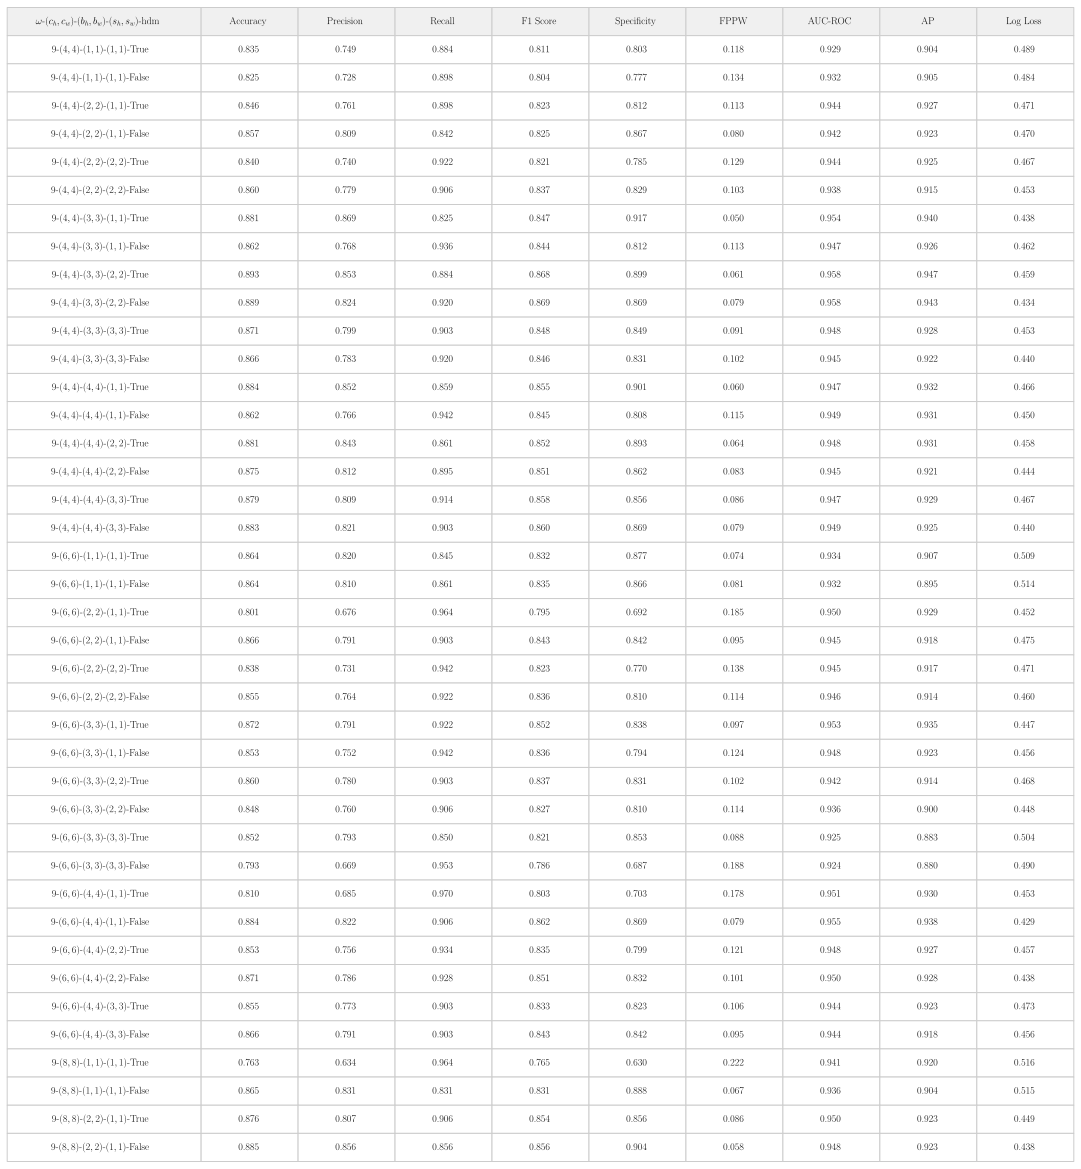
\includegraphics[width=\linewidth]{/Users/adamsam/repos/ee/Pedestrian-Detection/code/paper/tables/INRIA/INRIA_(100, 50)_0.png}
    \label{tab:INRIA_(100, 50)_0}
\end{table}

\begin{table}
    \caption{INRIA Results - (100, 50) Window}
    \includegraphics[width=\linewidth]{/Users/adamsam/repos/ee/Pedestrian-Detection/code/paper/tables/INRIA/INRIA_(100, 50)_120.png}
    \label{tab:INRIA_(100, 50)_120}
\end{table}

\begin{table}
    \caption{INRIA Results - (100, 50) Window}
    \includegraphics[width=\linewidth]{/Users/adamsam/repos/ee/Pedestrian-Detection/code/paper/tables/INRIA/INRIA_(100, 50)_160.png}
    \label{tab:INRIA_(100, 50)_160}
\end{table}

\begin{table}
    \caption{INRIA Results - (100, 50) Window}
    \includegraphics[width=\linewidth]{/Users/adamsam/repos/ee/Pedestrian-Detection/code/paper/tables/INRIA/INRIA_(100, 50)_200.png}
    \label{tab:INRIA_(100, 50)_200}
\end{table}

\begin{table}
    \caption{INRIA Results - (100, 50) Window}
    \includegraphics[width=\linewidth]{/Users/adamsam/repos/ee/Pedestrian-Detection/code/paper/tables/INRIA/INRIA_(100, 50)_40.png}
    \label{tab:INRIA_(100, 50)_40}
\end{table}

\begin{table}
    \caption{INRIA Results - (100, 50) Window}
    \includegraphics[width=\linewidth]{/Users/adamsam/repos/ee/Pedestrian-Detection/code/paper/tables/INRIA/INRIA_(100, 50)_80.png}
    \label{tab:INRIA_(100, 50)_80}
\end{table}

\subsubsection*{(112, 48) Window}

\begin{table}
    \caption{INRIA Results - (112, 48) Window}
    \includegraphics[width=\linewidth]{/Users/adamsam/repos/ee/Pedestrian-Detection/code/paper/tables/INRIA/INRIA_(112, 48)_0.png}
    \label{tab:INRIA_(112, 48)_0}
\end{table}

\begin{table}
    \caption{INRIA Results - (112, 48) Window}
    \includegraphics[width=\linewidth]{/Users/adamsam/repos/ee/Pedestrian-Detection/code/paper/tables/INRIA/INRIA_(112, 48)_120.png}
    \label{tab:INRIA_(112, 48)_120}
\end{table}

\begin{table}
    \caption{INRIA Results - (112, 48) Window}
    \includegraphics[width=\linewidth]{/Users/adamsam/repos/ee/Pedestrian-Detection/code/paper/tables/INRIA/INRIA_(112, 48)_160.png}
    \label{tab:INRIA_(112, 48)_160}
\end{table}

\begin{table}
    \caption{INRIA Results - (112, 48) Window}
    \includegraphics[width=\linewidth]{/Users/adamsam/repos/ee/Pedestrian-Detection/code/paper/tables/INRIA/INRIA_(112, 48)_200.png}
    \label{tab:INRIA_(112, 48)_200}
\end{table}

\begin{table}
    \caption{INRIA Results - (112, 48) Window}
    \includegraphics[width=\linewidth]{/Users/adamsam/repos/ee/Pedestrian-Detection/code/paper/tables/INRIA/INRIA_(112, 48)_40.png}
    \label{tab:INRIA_(112, 48)_40}
\end{table}

\begin{table}
    \caption{INRIA Results - (112, 48) Window}
    \includegraphics[width=\linewidth]{/Users/adamsam/repos/ee/Pedestrian-Detection/code/paper/tables/INRIA/INRIA_(112, 48)_80.png}
    \label{tab:INRIA_(112, 48)_80}
\end{table}

\subsubsection*{(128, 64) Window}

\begin{table}
    \caption{INRIA Results - (128, 64) Window}
    \includegraphics[width=\linewidth]{/Users/adamsam/repos/ee/Pedestrian-Detection/code/paper/tables/INRIA/INRIA_(128, 64)_0.png}
    \label{tab:INRIA_(128, 64)_0}
\end{table}

\begin{table}
    \caption{INRIA Results - (128, 64) Window}
    \includegraphics[width=\linewidth]{/Users/adamsam/repos/ee/Pedestrian-Detection/code/paper/tables/INRIA/INRIA_(128, 64)_120.png}
    \label{tab:INRIA_(128, 64)_120}
\end{table}

\begin{table}
    \caption{INRIA Results - (128, 64) Window}
    \includegraphics[width=\linewidth]{/Users/adamsam/repos/ee/Pedestrian-Detection/code/paper/tables/INRIA/INRIA_(128, 64)_160.png}
    \label{tab:INRIA_(128, 64)_160}
\end{table}

\begin{table}
    \caption{INRIA Results - (128, 64) Window}
    \includegraphics[width=\linewidth]{/Users/adamsam/repos/ee/Pedestrian-Detection/code/paper/tables/INRIA/INRIA_(128, 64)_200.png}
    \label{tab:INRIA_(128, 64)_200}
\end{table}

\begin{table}
    \caption{INRIA Results - (128, 64) Window}
    \includegraphics[width=\linewidth]{/Users/adamsam/repos/ee/Pedestrian-Detection/code/paper/tables/INRIA/INRIA_(128, 64)_40.png}
    \label{tab:INRIA_(128, 64)_40}
\end{table}

\begin{table}
    \caption{INRIA Results - (128, 64) Window}
    \includegraphics[width=\linewidth]{/Users/adamsam/repos/ee/Pedestrian-Detection/code/paper/tables/INRIA/INRIA_(128, 64)_80.png}
    \label{tab:INRIA_(128, 64)_80}
\end{table}

\subsubsection*{(128, 96) Window}

\begin{table}
    \caption{INRIA Results - (128, 96) Window}
    \includegraphics[width=\linewidth]{/Users/adamsam/repos/ee/Pedestrian-Detection/code/paper/tables/INRIA/INRIA_(128, 96)_0.png}
    \label{tab:INRIA_(128, 96)_0}
\end{table}

\begin{table}
    \caption{INRIA Results - (128, 96) Window}
    \includegraphics[width=\linewidth]{/Users/adamsam/repos/ee/Pedestrian-Detection/code/paper/tables/INRIA/INRIA_(128, 96)_120.png}
    \label{tab:INRIA_(128, 96)_120}
\end{table}

\begin{table}
    \caption{INRIA Results - (128, 96) Window}
    \includegraphics[width=\linewidth]{/Users/adamsam/repos/ee/Pedestrian-Detection/code/paper/tables/INRIA/INRIA_(128, 96)_160.png}
    \label{tab:INRIA_(128, 96)_160}
\end{table}

\begin{table}
    \caption{INRIA Results - (128, 96) Window}
    \includegraphics[width=\linewidth]{/Users/adamsam/repos/ee/Pedestrian-Detection/code/paper/tables/INRIA/INRIA_(128, 96)_200.png}
    \label{tab:INRIA_(128, 96)_200}
\end{table}

\begin{table}
    \caption{INRIA Results - (128, 96) Window}
    \includegraphics[width=\linewidth]{/Users/adamsam/repos/ee/Pedestrian-Detection/code/paper/tables/INRIA/INRIA_(128, 96)_40.png}
    \label{tab:INRIA_(128, 96)_40}
\end{table}

\begin{table}
    \caption{INRIA Results - (128, 96) Window}
    \includegraphics[width=\linewidth]{/Users/adamsam/repos/ee/Pedestrian-Detection/code/paper/tables/INRIA/INRIA_(128, 96)_80.png}
    \label{tab:INRIA_(128, 96)_80}
\end{table}

\subsubsection{Caltech Score Tables}

\subsubsection*{(100, 50)$\times$(100, 50) Window}

\begin{table}
    \caption{caltech Results - (100, 50)$\times$(100, 50) Window}
    \includegraphics[width=\linewidth]{/Users/adamsam/repos/ee/Pedestrian-Detection/code/paper/tables/caltech_30/caltech_30_(100, 50)_0.png}
    \label{tab:caltech_30_(100, 50)_0}
\end{table}

\begin{table}
    \caption{caltech Results - (100, 50)$\times$(100, 50) Window}
    \includegraphics[width=\linewidth]{/Users/adamsam/repos/ee/Pedestrian-Detection/code/paper/tables/caltech_30/caltech_30_(100, 50)_120.png}
    \label{tab:caltech_30_(100, 50)_120}
\end{table}

\begin{table}
    \caption{caltech Results - (100, 50)$\times$(100, 50) Window}
    \includegraphics[width=\linewidth]{/Users/adamsam/repos/ee/Pedestrian-Detection/code/paper/tables/caltech_30/caltech_30_(100, 50)_160.png}
    \label{tab:caltech_30_(100, 50)_160}
\end{table}

\begin{table}
    \caption{caltech Results - (100, 50)$\times$(100, 50) Window}
    \includegraphics[width=\linewidth]{/Users/adamsam/repos/ee/Pedestrian-Detection/code/paper/tables/caltech_30/caltech_30_(100, 50)_200.png}
    \label{tab:caltech_30_(100, 50)_200}
\end{table}

\begin{table}
    \caption{caltech Results - (100, 50)$\times$(100, 50) Window}
    \includegraphics[width=\linewidth]{/Users/adamsam/repos/ee/Pedestrian-Detection/code/paper/tables/caltech_30/caltech_30_(100, 50)_40.png}
    \label{tab:caltech_30_(100, 50)_40}
\end{table}

\begin{table}
    \caption{caltech Results - (100, 50)$\times$(100, 50) Window}
    \includegraphics[width=\linewidth]{/Users/adamsam/repos/ee/Pedestrian-Detection/code/paper/tables/caltech_30/caltech_30_(100, 50)_80.png}
    \label{tab:caltech_30_(100, 50)_80}
\end{table}

\subsubsection*{(112, 48)$\times$(112, 48) Window}

\begin{table}
    \caption{caltech Results - (112, 48)$\times$(112, 48) Window}
    \includegraphics[width=\linewidth]{/Users/adamsam/repos/ee/Pedestrian-Detection/code/paper/tables/caltech_30/caltech_30_(112, 48)_0.png}
    \label{tab:caltech_30_(112, 48)_0}
\end{table}

\begin{table}
    \caption{caltech Results - (112, 48)$\times$(112, 48) Window}
    \includegraphics[width=\linewidth]{/Users/adamsam/repos/ee/Pedestrian-Detection/code/paper/tables/caltech_30/caltech_30_(112, 48)_120.png}
    \label{tab:caltech_30_(112, 48)_120}
\end{table}

\begin{table}
    \caption{caltech Results - (112, 48)$\times$(112, 48) Window}
    \includegraphics[width=\linewidth]{/Users/adamsam/repos/ee/Pedestrian-Detection/code/paper/tables/caltech_30/caltech_30_(112, 48)_160.png}
    \label{tab:caltech_30_(112, 48)_160}
\end{table}

\begin{table}
    \caption{caltech Results - (112, 48)$\times$(112, 48) Window}
    \includegraphics[width=\linewidth]{/Users/adamsam/repos/ee/Pedestrian-Detection/code/paper/tables/caltech_30/caltech_30_(112, 48)_200.png}
    \label{tab:caltech_30_(112, 48)_200}
\end{table}

\begin{table}
    \caption{caltech Results - (112, 48)$\times$(112, 48) Window}
    \includegraphics[width=\linewidth]{/Users/adamsam/repos/ee/Pedestrian-Detection/code/paper/tables/caltech_30/caltech_30_(112, 48)_40.png}
    \label{tab:caltech_30_(112, 48)_40}
\end{table}

\begin{table}
    \caption{caltech Results - (112, 48)$\times$(112, 48) Window}
    \includegraphics[width=\linewidth]{/Users/adamsam/repos/ee/Pedestrian-Detection/code/paper/tables/caltech_30/caltech_30_(112, 48)_80.png}
    \label{tab:caltech_30_(112, 48)_80}
\end{table}

\subsubsection*{(128, 64)$\times$(128, 64) Window}

\begin{table}
    \caption{caltech Results - (128, 64)$\times$(128, 64) Window}
    \includegraphics[width=\linewidth]{/Users/adamsam/repos/ee/Pedestrian-Detection/code/paper/tables/caltech_30/caltech_30_(128, 64)_0.png}
    \label{tab:caltech_30_(128, 64)_0}
\end{table}

\begin{table}
    \caption{caltech Results - (128, 64)$\times$(128, 64) Window}
    \includegraphics[width=\linewidth]{/Users/adamsam/repos/ee/Pedestrian-Detection/code/paper/tables/caltech_30/caltech_30_(128, 64)_120.png}
    \label{tab:caltech_30_(128, 64)_120}
\end{table}

\begin{table}
    \caption{caltech Results - (128, 64)$\times$(128, 64) Window}
    \includegraphics[width=\linewidth]{/Users/adamsam/repos/ee/Pedestrian-Detection/code/paper/tables/caltech_30/caltech_30_(128, 64)_160.png}
    \label{tab:caltech_30_(128, 64)_160}
\end{table}

\begin{table}
    \caption{caltech Results - (128, 64)$\times$(128, 64) Window}
    \includegraphics[width=\linewidth]{/Users/adamsam/repos/ee/Pedestrian-Detection/code/paper/tables/caltech_30/caltech_30_(128, 64)_200.png}
    \label{tab:caltech_30_(128, 64)_200}
\end{table}

\begin{table}
    \caption{caltech Results - (128, 64)$\times$(128, 64) Window}
    \includegraphics[width=\linewidth]{/Users/adamsam/repos/ee/Pedestrian-Detection/code/paper/tables/caltech_30/caltech_30_(128, 64)_40.png}
    \label{tab:caltech_30_(128, 64)_40}
\end{table}

\begin{table}
    \caption{caltech Results - (128, 64)$\times$(128, 64) Window}
    \includegraphics[width=\linewidth]{/Users/adamsam/repos/ee/Pedestrian-Detection/code/paper/tables/caltech_30/caltech_30_(128, 64)_80.png}
    \label{tab:caltech_30_(128, 64)_80}
\end{table}

\subsubsection*{(128, 96)$\times$(128, 96) Window}

\begin{table}
    \caption{caltech Results - (128, 96)$\times$(128, 96) Window}
    \includegraphics[width=\linewidth]{/Users/adamsam/repos/ee/Pedestrian-Detection/code/paper/tables/caltech_30/caltech_30_(128, 96)_0.png}
    \label{tab:caltech_30_(128, 96)_0}
\end{table}

\begin{table}
    \caption{caltech Results - (128, 96)$\times$(128, 96) Window}
    \includegraphics[width=\linewidth]{/Users/adamsam/repos/ee/Pedestrian-Detection/code/paper/tables/caltech_30/caltech_30_(128, 96)_120.png}
    \label{tab:caltech_30_(128, 96)_120}
\end{table}

\begin{table}
    \caption{caltech Results - (128, 96)$\times$(128, 96) Window}
    \includegraphics[width=\linewidth]{/Users/adamsam/repos/ee/Pedestrian-Detection/code/paper/tables/caltech_30/caltech_30_(128, 96)_160.png}
    \label{tab:caltech_30_(128, 96)_160}
\end{table}

\begin{table}
    \caption{caltech Results - (128, 96)$\times$(128, 96) Window}
    \includegraphics[width=\linewidth]{/Users/adamsam/repos/ee/Pedestrian-Detection/code/paper/tables/caltech_30/caltech_30_(128, 96)_200.png}
    \label{tab:caltech_30_(128, 96)_200}
\end{table}

\begin{table}
    \caption{caltech Results - (128, 96)$\times$(128, 96) Window}
    \includegraphics[width=\linewidth]{/Users/adamsam/repos/ee/Pedestrian-Detection/code/paper/tables/caltech_30/caltech_30_(128, 96)_40.png}
    \label{tab:caltech_30_(128, 96)_40}
\end{table}

\begin{table}
    \caption{caltech Results - (128, 96)$\times$(128, 96) Window}
    \includegraphics[width=\linewidth]{/Users/adamsam/repos/ee/Pedestrian-Detection/code/paper/tables/caltech_30/caltech_30_(128, 96)_80.png}
    \label{tab:caltech_30_(128, 96)_80}
\end{table}

\subsubsection{PnPLO Score Tables}

\subsubsection*{(100, 50) Window}

\begin{table}
    \caption{PnPLO Results - (100, 50) Window}
    \includegraphics[width=\linewidth]{/Users/adamsam/repos/ib/ee/Pedestrian-Detection/code/paper/tables/PnPLO/PnPLO_(100, 50)_0.png}
    \label{tab:PnPLO_(100, 50)_0}
\end{table}

\begin{table}
    \caption{PnPLO Results - (100, 50) Window}
    \includegraphics[width=\linewidth]{/Users/adamsam/repos/ib/ee/Pedestrian-Detection/code/paper/tables/PnPLO/PnPLO_(100, 50)_120.png}
    \label{tab:PnPLO_(100, 50)_120}
\end{table}

\begin{table}
    \caption{PnPLO Results - (100, 50) Window}
    \includegraphics[width=\linewidth]{/Users/adamsam/repos/ib/ee/Pedestrian-Detection/code/paper/tables/PnPLO/PnPLO_(100, 50)_160.png}
    \label{tab:PnPLO_(100, 50)_160}
\end{table}

\begin{table}
    \caption{PnPLO Results - (100, 50) Window}
    \includegraphics[width=\linewidth]{/Users/adamsam/repos/ib/ee/Pedestrian-Detection/code/paper/tables/PnPLO/PnPLO_(100, 50)_200.png}
    \label{tab:PnPLO_(100, 50)_200}
\end{table}

\begin{table}
    \caption{PnPLO Results - (100, 50) Window}
    \includegraphics[width=\linewidth]{/Users/adamsam/repos/ib/ee/Pedestrian-Detection/code/paper/tables/PnPLO/PnPLO_(100, 50)_40.png}
    \label{tab:PnPLO_(100, 50)_40}
\end{table}

\begin{table}
    \caption{PnPLO Results - (100, 50) Window}
    \includegraphics[width=\linewidth]{/Users/adamsam/repos/ib/ee/Pedestrian-Detection/code/paper/tables/PnPLO/PnPLO_(100, 50)_80.png}
    \label{tab:PnPLO_(100, 50)_80}
\end{table}

\subsubsection*{(112, 48) Window}

\begin{table}
    \caption{PnPLO Results - (112, 48) Window}
    \includegraphics[width=\linewidth]{/Users/adamsam/repos/ib/ee/Pedestrian-Detection/code/paper/tables/PnPLO/PnPLO_(112, 48)_0.png}
    \label{tab:PnPLO_(112, 48)_0}
\end{table}

\begin{table}
    \caption{PnPLO Results - (112, 48) Window}
    \includegraphics[width=\linewidth]{/Users/adamsam/repos/ib/ee/Pedestrian-Detection/code/paper/tables/PnPLO/PnPLO_(112, 48)_120.png}
    \label{tab:PnPLO_(112, 48)_120}
\end{table}

\begin{table}
    \caption{PnPLO Results - (112, 48) Window}
    \includegraphics[width=\linewidth]{/Users/adamsam/repos/ib/ee/Pedestrian-Detection/code/paper/tables/PnPLO/PnPLO_(112, 48)_160.png}
    \label{tab:PnPLO_(112, 48)_160}
\end{table}

\begin{table}
    \caption{PnPLO Results - (112, 48) Window}
    \includegraphics[width=\linewidth]{/Users/adamsam/repos/ib/ee/Pedestrian-Detection/code/paper/tables/PnPLO/PnPLO_(112, 48)_200.png}
    \label{tab:PnPLO_(112, 48)_200}
\end{table}

\begin{table}
    \caption{PnPLO Results - (112, 48) Window}
    \includegraphics[width=\linewidth]{/Users/adamsam/repos/ib/ee/Pedestrian-Detection/code/paper/tables/PnPLO/PnPLO_(112, 48)_40.png}
    \label{tab:PnPLO_(112, 48)_40}
\end{table}

\begin{table}
    \caption{PnPLO Results - (112, 48) Window}
    \includegraphics[width=\linewidth]{/Users/adamsam/repos/ib/ee/Pedestrian-Detection/code/paper/tables/PnPLO/PnPLO_(112, 48)_80.png}
    \label{tab:PnPLO_(112, 48)_80}
\end{table}

\subsubsection*{(128, 64) Window}

\begin{table}
    \caption{PnPLO Results - (128, 64) Window}
    \includegraphics[width=\linewidth]{/Users/adamsam/repos/ib/ee/Pedestrian-Detection/code/paper/tables/PnPLO/PnPLO_(128, 64)_0.png}
    \label{tab:PnPLO_(128, 64)_0}
\end{table}

\begin{table}
    \caption{PnPLO Results - (128, 64) Window}
    \includegraphics[width=\linewidth]{/Users/adamsam/repos/ib/ee/Pedestrian-Detection/code/paper/tables/PnPLO/PnPLO_(128, 64)_120.png}
    \label{tab:PnPLO_(128, 64)_120}
\end{table}

\begin{table}
    \caption{PnPLO Results - (128, 64) Window}
    \includegraphics[width=\linewidth]{/Users/adamsam/repos/ib/ee/Pedestrian-Detection/code/paper/tables/PnPLO/PnPLO_(128, 64)_160.png}
    \label{tab:PnPLO_(128, 64)_160}
\end{table}

\begin{table}
    \caption{PnPLO Results - (128, 64) Window}
    \includegraphics[width=\linewidth]{/Users/adamsam/repos/ib/ee/Pedestrian-Detection/code/paper/tables/PnPLO/PnPLO_(128, 64)_200.png}
    \label{tab:PnPLO_(128, 64)_200}
\end{table}

\begin{table}
    \caption{PnPLO Results - (128, 64) Window}
    \includegraphics[width=\linewidth]{/Users/adamsam/repos/ib/ee/Pedestrian-Detection/code/paper/tables/PnPLO/PnPLO_(128, 64)_40.png}
    \label{tab:PnPLO_(128, 64)_40}
\end{table}

\begin{table}
    \caption{PnPLO Results - (128, 64) Window}
    \includegraphics[width=\linewidth]{/Users/adamsam/repos/ib/ee/Pedestrian-Detection/code/paper/tables/PnPLO/PnPLO_(128, 64)_80.png}
    \label{tab:PnPLO_(128, 64)_80}
\end{table}

\subsubsection*{(128, 96) Window}

\begin{table}
    \caption{PnPLO Results - (128, 96) Window}
    \includegraphics[width=\linewidth]{/Users/adamsam/repos/ib/ee/Pedestrian-Detection/code/paper/tables/PnPLO/PnPLO_(128, 96)_0.png}
    \label{tab:PnPLO_(128, 96)_0}
\end{table}

\begin{table}
    \caption{PnPLO Results - (128, 96) Window}
    \includegraphics[width=\linewidth]{/Users/adamsam/repos/ib/ee/Pedestrian-Detection/code/paper/tables/PnPLO/PnPLO_(128, 96)_120.png}
    \label{tab:PnPLO_(128, 96)_120}
\end{table}

\begin{table}
    \caption{PnPLO Results - (128, 96) Window}
    \includegraphics[width=\linewidth]{/Users/adamsam/repos/ib/ee/Pedestrian-Detection/code/paper/tables/PnPLO/PnPLO_(128, 96)_160.png}
    \label{tab:PnPLO_(128, 96)_160}
\end{table}

\begin{table}
    \caption{PnPLO Results - (128, 96) Window}
    \includegraphics[width=\linewidth]{/Users/adamsam/repos/ib/ee/Pedestrian-Detection/code/paper/tables/PnPLO/PnPLO_(128, 96)_200.png}
    \label{tab:PnPLO_(128, 96)_200}
\end{table}

\begin{table}
    \caption{PnPLO Results - (128, 96) Window}
    \includegraphics[width=\linewidth]{/Users/adamsam/repos/ib/ee/Pedestrian-Detection/code/paper/tables/PnPLO/PnPLO_(128, 96)_40.png}
    \label{tab:PnPLO_(128, 96)_40}
\end{table}

\begin{table}
    \caption{PnPLO Results - (128, 96) Window}
    \includegraphics[width=\linewidth]{/Users/adamsam/repos/ib/ee/Pedestrian-Detection/code/paper/tables/PnPLO/PnPLO_(128, 96)_80.png}
    \label{tab:PnPLO_(128, 96)_80}
\end{table}

\input{}